\documentclass[conference]{IEEEtran}
\usepackage[justification=centering]{caption}
\usepackage{blindtext, graphicx}
\usepackage{float}

\begin{document}
\title{Three Approaches to a Team Building Application}

\author{\IEEEauthorblockN{Michael Goff\IEEEauthorrefmark{1},
Shashank Jha\IEEEauthorrefmark{2},
Jingjuan Deng\IEEEauthorrefmark{3} and
Bhaskar Sinha\IEEEauthorrefmark{4}}
\IEEEauthorblockA{Department of Computer Science, North Carolina State University, \\
Raleigh, North Carolina 27606\\ 
Email: \IEEEauthorrefmark{1}magoff2@ncsu.edu \\
\IEEEauthorrefmark{2}sjha5@ncsu.edu \\
\IEEEauthorrefmark{3}jdeng8@ncsu.edu \\
\IEEEauthorrefmark{4}bsinha@ncsu.edu}}


% make the title area
\maketitle

\section{Abstract}
Every now and then students from every discipline have to team up for group projects. The success of the projects could depend on various factors such as the skills of the students partaking, social compatibility, matching schedule, interests, past experience. Through our project we have aimed to facilitate the process of team division based on skills or expertise in different facets of software development such as front-end, back-end, database. For the same, we have created three different applications using Google's Firebase and AngularJS. We then conducted experiments to compare all three approaches and asked users for feedback for further improvements.      
\section{Keywords}
Team division, balanced teams, joining team, creating team

\section{Introduction}
After presenting our idea to the SE class and doing user evaluation sessions, we concluded that building a team creation application is definitely worth a go. Out of all the factors which contributes to a team successfully working together, we decided to concentrate on skill-set division. Hence, our first approach was to allow users to search for other users with a particular skill set which they require in their project. Second approach was intended for the professor, where they already have a list of users and their expertise areas and with one press of button, they can create multiple teams with balanced expertise. Third approach was allowing user to join only those teams which has positions matching their expertise.
In this paper, we first discuss the experiments which we did as part of evaluation and the response of the participants. After that we explain all three approaches and improvements which we can make in them based on user feedback. Finally, we conclude which one is the best approach among three and what can be done to take the project further in future.

\section{Experiment}
This section will outline the parts of the experiment we conducted with our participants during individual sessions held at Hunt Library.

\subsection{Task Methodology}
For each approach, we designed scenarios for users to use the application. Approach 1 and 3 are student based applications, we evaluate them by user's experience. 

In order to prove the value of automated group sorting in approach 2 we created a list of 20 randomly generated users with varying expertise in front-end, back-end and database development. We gave each participant a blank sheet of paper and asked them to sort the users into balanced groups based off of the available skills. We intentionally neglected to provide any further direction so we could see what the thought process would be as they wrote the teams on the paper. We also tracked the time it took to complete the formation of teams. 

After having the participants manually sort through the table of users we had them log into an account on the team generation web-page and allowed them to generate the teams automatically using the same set of users that were also inserted into the database. We noted the time from logging in to arriving at the generated teams page.

Following the experiment for the second approach we had the participant fill out a Google form with some survey questions to get a feel of their impressions. We asked "Is it clear to you what approach 2 does and its purpose?" in order to confirm that users understood the point of the application. We asked "Is it easy to perform the basic functions of approach 2" and "If you had to use approach 2 again would you need assistance or support?" to make sure that the usability was good for the second approach. We asked if the user felt that approach 2 made it easier to create teams and to rate the overall experience to make sure that the application was useful to the user. Finally we asked what improvements they suggested for the application. We made this an open ended question so we could get broad feedback about the application. 

In approach 3, we created a list of teams, in which there are positions with required skills. Some positions are already applied and not available to other users. After users signing up to the application, they can edit their profiles and skills. When users want to join a team, they go to the teams page, which shows the basic condition of existing teams. Then users can choose from available positions according to their skills set in the profile. They can only applied for positions which are available and fitting for their skills since the applied button will not show up if a user doesn't meet the requirements. After joining a team, users go to the team information page to see who are their team members and the contact information. If users change their minds, they go to the teams page, quit from the current team and join another team. 

After showing users the basic operations, we ask them to try the application then help filling up our questionnaire. The questionnaire evaluates whether the application achieves its purpose, its usability and the overall user experience. Also we compare the three approaches to find their pros and cons, to figure out which approach is the best.

\subsection{Participants}
We chose participants who were graduate students at North Carolina State University from the Software Engineering class. All participants came to in person sessions where we walked them through the applications in order to assess their feedback in person. 

Before starting the demos, we wanted to collect background information about the participants. We asked them if they thought skill was an important factor in deciding a team's performance to which 96\% of respondents responded yes. The point of this question was to make sure that these participants shared our view that skills were one of the most important factors in developing a strong team since we based our entire applications around this idea. 

We also asked the participants if they had the ability to choose team members based off of their skills if it would be helpful to them. We found that 100\% of respondents responded yes to this question, proving that skills are certainly an important factor in creating a good team. 


\section{Results}
In approach 2 the results of the timing activity were pretty much as expected. Out of 25 participants the time to sort the 20 users manually into balanced groups based off of their skills took an average of 3 minutes and 55 seconds. When logging into the application and selecting generate groups the participants took an average of 12.92 seconds to complete the activity. So it is significantly faster to let the computer do the sorting for you to a factor of about 18 times faster. 

We were surprised to see that almost all of the manual responses had very similar group setups when the activity was complete. We think that it might have something to do with just going in order down the list filling in each group as you go. Unsurprisingly, this was very similar to the group structure the application took as well so the performance of each was comparable. The time difference is what really stands out in automating team creation.

The results for the survey were positive for the second approach as well. When asked whether the application's purpose was clear, 100\% of respondents answered yes. All of the respondents also said yes to the question of whether it was was easy to perform the basic functions of the application. However, only 84\% of respondents said they would not need assistance to use the application again. Fortunately, 100\% of people agreed that the application made it easier to form balanced teams, which was our intent with the application. Finally, the user experience looks good, on a scale of 1 to 5 for user experience, 84\% of users rated it as a 5 and the remainder rated it as a 4 on user experience. 

Users' experience of approach 3 is good. All of the participants think this approach achieves the purpose of creating teams. And most of them(88\%) think it can create skill-balanced teams. 76\% of our users need no help and assistance in the future use(Fig.\ref{app3.ua}) , but there are still 24\% users think this application is hard to use. Among 25 participants, 60\% give full marks(5) on user experience, 24\% rate it 4 and the left 16\% rate it 3.(Fig.\ref{app3.ov}) 

\begin{figure}[H]
    \centering
    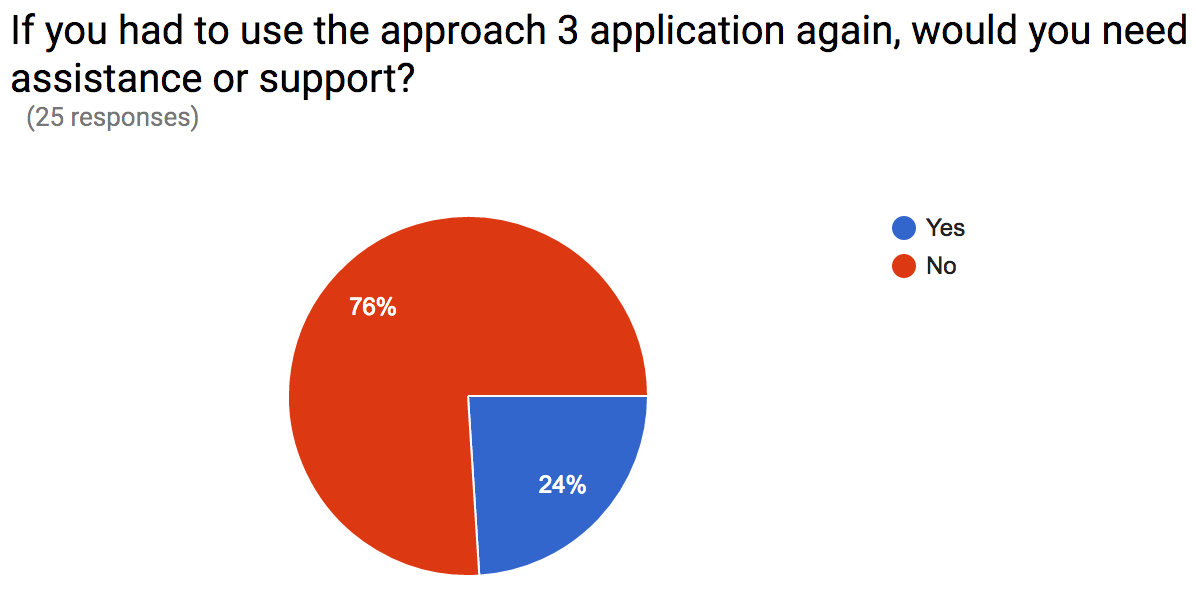
\includegraphics[width=9cm]{image/app3_useagain.png}
    \caption{Need assistance to use approach 3}
    \label{app3.ua}
\end{figure}

\begin{figure}[H]
    \centering
    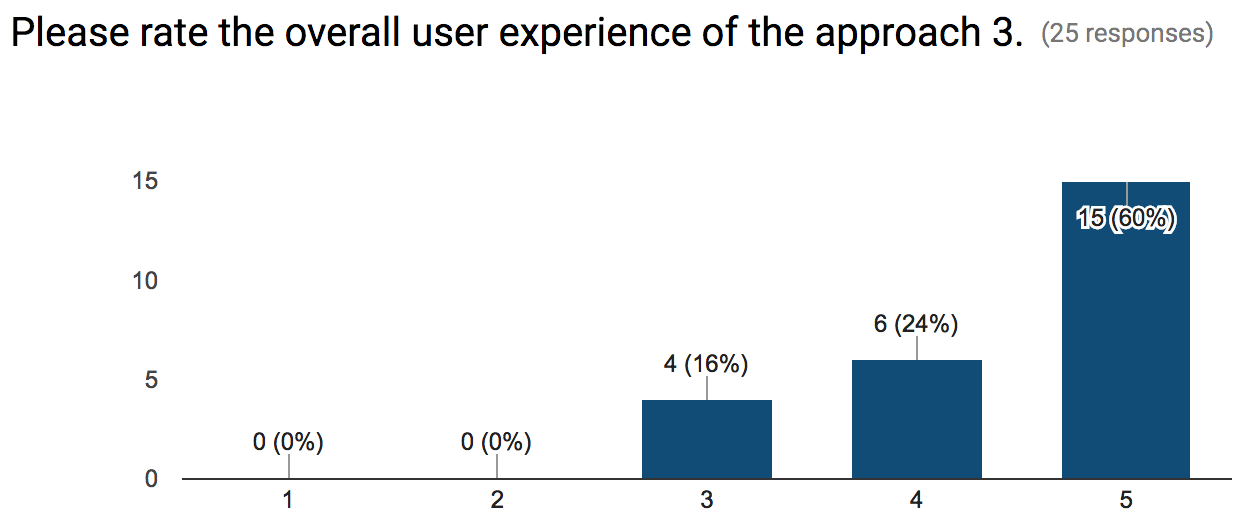
\includegraphics[width=9cm]{image/app3_overall.png}
    \caption{The overall user experience of approach 3}
    \label{app3.ov}
\end{figure}

We ask users questions about  which features they like in approach 3 (multiple choices). The result is showed in Fig.\ref{app3.gf}, Joining teams freely and A glance on teams information are the two most popular answers. Among all participants, over 80\%(20 of 25 participants) of them like these two features. The third popular answer is Offering contact information of team members, about 60\% users choose this feature. Quitting from a team and competing for positions in time is the least two popular features, there are over 50\% users like these features.

\begin{figure}[H]
    \centering
    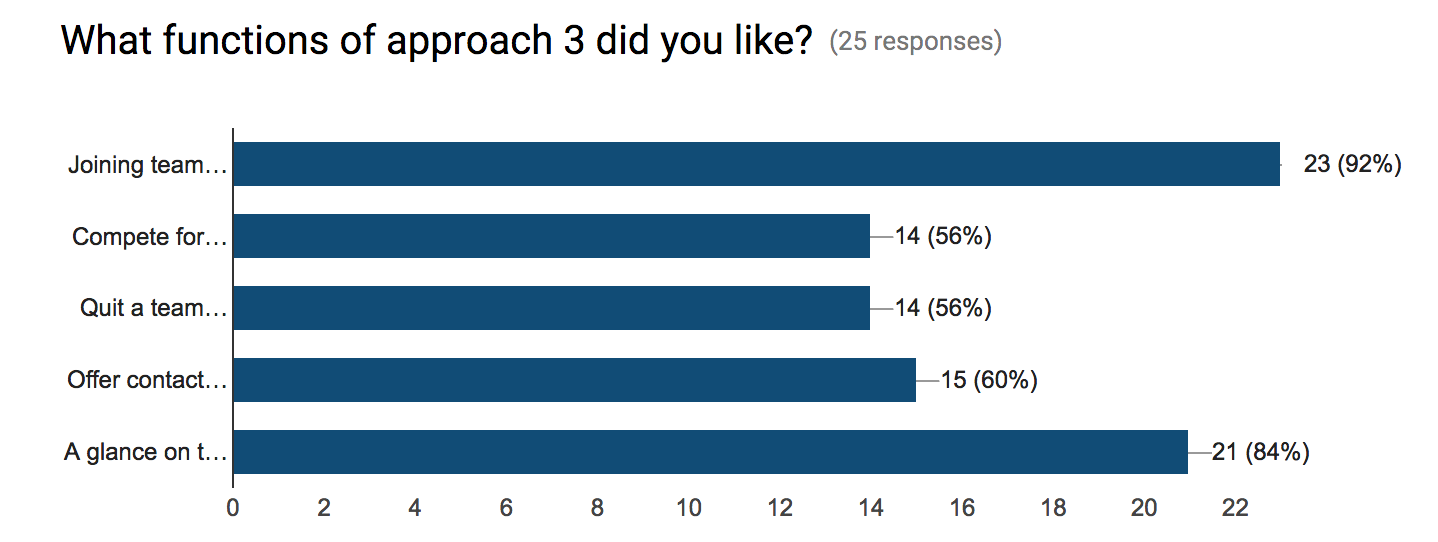
\includegraphics[width=9cm]{image/app3_goodfeatures.png}
    \caption{Good features of approach 3}
    \label{app3.gf}
\end{figure}

\section{Discussion}
After conducting user evaluations and collecting results we were able to arrive at a plethora of conclusions about our applications. The most obvious being that we have plenty of room for improvement on the layout and flow of our applications. When we were working on each application separately we all took different design paths which lead to some confusion among participants on how to use the various features. We were already aware of some smaller issues, since we only had a limited development time and a workable prototype was okay, but introducing unbiased users into the system revealed a lot more issues than what was on the surface. 

Within this section, we will discuss the key points about each approach especially the strengths and weaknesses of each one. In order to draw these conclusions, we will synthesis the data from the survey with the primary focus on the short answer responses, since that is where the respondents were allowed the most freedom in their opinions. 

\subsection{Observations / Limitations}

\subsection{Approach 1: Skill based searching}

\subsection{Approach 2: Automated Sorting}
Approach 2 was the most hands-off approach for the user since the machine does most of the work on the user's behalf. This made it more difficult to give a traditional tour of the application since there was pretty much only one button for the user to press when acting as the role of the professor. However, the results were exactly what was expected. The application successfully created balanced teams at the push of a button that were on par with the teams that were formed manually by survey participants and in a fraction of the time. 

When we asked the users about what improvements could be made to the second approach we got a lot of great responses back. We were pleased to find out that most of the responses were compliments including that it was perfect and that it was well developed, both of which are great signs for the usability of the application. In addition to praise, a lot of the responses were smaller nitpicks about the application itself, like to add the names to the sorted teams page, a small detail we forgot to add in implementation. Other suggestions included, adding a scale of proficiency for the skill categories or even the introduction of a Testing category for required skills in a team. Both of these suggestions are great recommendations to improve the quality of the application that were not even considered at all during development. When you introduce weighted proficiencies in multiple skills you can allow the system to more intelligently place you into a group under a skill that you are stronger with rather than one that you have just learned. It also avoids the binary approach to either knowing something or not since that can vary based on the subject's own opinion of their skills. The Testing category is another great addition since it is another broad category and does not fit well underneath any of the other existing skills. 

A lot of participants suggested to break the categories down into a more granular approach of skills similar to approach 1. While having more information about each user is generally a good thing we think that keep the categories broad is more appropriate for a project environment. It would be much harder to sort groups based off of a wide skill pool since it would be nearly impossible to create balanced groups. At least within each broad skill category the thought process would translate easier across arbitrary languages. Since the languages are not defined for projects the idea of transferable skills were more preferred. School always preaches that you shouldn't learn the language but rather the concept. 

One final preference was to add the ability for the professor to tweak the results. We thought this was a great idea because the professor will always know the class better than the computer does and will already have some idea of how well certain students may work together. In order to implement this, we should let each row in the team table be draggable which will allow for a professor to slide a student from one group to another however they want. 

Overall, the second approach was pretty popular among survey respondents, there were a number of great suggestions that were not previously considered which is great insight for future development on these applications. When we asked users for their reasoning behind picking their favorite application, the respondents had a lot of good insight about approach 2. The most popular opinions were that it was fast and random which allowed busy students to quickly find teams that were automatically balanced. So when students don't mind meeting new people and quickly getting into a team without any extra work on their part, the automated team creation application definitely shines. 

\subsection{Approach 3: Joining existing teams}
Approach 3 is similar to the course selection process in college. Users must satisfy the skill requirement of specific position. The positions in a team is limited, so if one team is full, users have to choose other teams. 

Since the skills and positions in each team are fixed, this approach is designed to guarantee creating skill-balanced teams, which is the primarily concern of our project. But few of the users think it is not easy to create skill-balance teams. We want to figure out the reason. For approach 3 evaluation, we focus on:(1) how is user experience (2) what happens during team formation affect user experience and (3) what changes we can make to improve it.

According to the survey, we find that for the users who choose approach 3, most of them give two main reasons. One is this approach offers information about overall teams condition and team mates' contact information. In order to create user-satisfied teams, users need information about current teams formation, how many positions left, what positions they can compete for and members' details in each team. These information help them making better decisions when joining or quitting a team. 

Although we offer useful information of teams formation and position availabilities before users selecting their teams, the approach is lack of information about the details of team members in each team. Some users think it's better to have these information when making team joining decisions. This is one drawback of approach 3, while approach 1 provides detailed individual information. A better way to solve this is combining the advantages of approach 1 and 3.

Another advantages of approach 3 is that they can join a team or quit from a team whenever they want. Compare to approach 2, approach 3 gives users freedom when selecting teams or changing their minds. However, some users think this freedom might cause some problems. Imagine that if users keep changing their minds, teams will never settle down. One improvement on this problem is setting some constraints on changing team actions. For an example, adding time limit on joining and quiting teams. In the time limit, user can compare teams and choose which team they fit the most. When it exceeds time limit, users can not change their team status anymore, which keeps the teams formation more stable.

Due to trading off between time and implementation, approach 3 have some drawbacks. Several users asked for improvements on UI in approach 3. One question in our questionnaire is If you had to use the approach 3 application again, would you need assistance or support?(Fig.\ref{app3.ua}) About 24\% of participants required assistance in the future use. We realized that non-functional requirements like interface friendly and usability are also important factor affect user experience.

 \begin{table}[!htb]\centering
 \begin{tabular} { | c | c |  c |}
 \hline
&pros & cons\\
 \hline
1& clear and concise & UI unfriendly\\
 \hline
2& overall team information & lack of detailed information\\
 \hline
3&join or quit freely & team breaks easily\\
 \hline
 \end{tabular}
 \caption{Pros and cons of approach 3}
 \end{table}

In all, approach 3 get good feedback in evaluation because it offers convenience, free choices and some useful information for users to form teams. About one of third users prefer to use approach 3 to solve team formation problem. The primary drawbacks which affect users' experience are UI, quiting constraints and lack of teammates' information before selecting a team. 


\subsection{Best Approach}
\blindtext


\section{Conclusion}
All three of our approaches were different and each of them assisted users to form better teams in their own. While approach1 made the owner of the project in driving seat, approach3 gave the users option to join a team. Approach2 would be ideal for professors who want students to have experience of working with random people. Though students are not appreciative of this idea, this is what happens in office or post-school term. Since we had three different and independent approaches, we were expecting one to be better than other. Also, as our evaluators were fellow SE students, we expected approach1 or approach3 to be winner. Both these approaches were student based and approach2 was professor based. We thought that approach2 would be favored only by professors who like dividing the team randomly. Surprisingly, all three approaches got similar amount of votes. This further reiterates our belief that if skills are divided evenly among teams, students are willing to work with new people as well.

//Will be adding more lines based on individual approaches 

\section{Future Work}
Since we did not have any clear winner among three approaches, we believe that best way forward would be to combine all three approaches into single application. All three approaches already have common starting point, i.e., signing up and adding your skill sets. We could also ask users to provide their LinkedIn profile. Next step would be to ask if the user wants to add new project or check existing ones. If he decides to create new project, he can list that as open or close. If it is a closed project, then he needs to contact other persons for forming the team (approach1). An open project would mean that other users can see that project and apply if they have desired skills (approach3). This would be same as user selecting 'check existing projects' and then joining team. For approach2, user needs to join a list shared by professor. Professor can then divide the list into further teams after a deadline (approach2). Having roles defined will make sure that only professor is able to generate teams. Currently, all the users have the ability to generate teams. So one single application can cover all the approaches.  

Though our application is targeted for students and professors, it can easily be extended to cover professional employees and their managers as well. Approach3 would be ideal for crowd sourcing. User would create project and others would be able to join the project if they have desired skills. Since approach3 does not give the project owner any control of who joins the team, it would be best suited for crowd sourcing. 


\end{document}